\subsection{The Stochastic Representation by Gaussian Processes}
Let $s(t)$ for $t\in [0,\infty]$ be a continuous signal which is observed on discrete grid of points in the interval $[0,T]$. We consider not so uncommon situation, when the observed values of $s(t)$ are perturbed by some noise component. The perturbation of the true signal can be either deterministic or stochastic. The deterministic noise might be a results of  a chaotic 


 and therefore the process which we observe is in fact
\begin{equation}\label{eq:signal_noisy_y}
y(t) = s(t) + \epsilon, \text{ for } \epsilon \in \mathcal{N}(0, \sigma^2).
\end{equation}
Therefore, our observation set consist of the pairs $\big\{t_n,y_n\big\}$ where $y_n = y(t_n)$ for $t_n \in [0,T]$. Let us remark that for the same

 the realisations of the continuous signal $s(t)$ on the discrete sent of points. W


Let $x(t)$ be a continuous real-valued signal which is an approximation of the signal $s(t)$ based on its observed values. Therefore, $x(t)$ is  

and let us define its EMD decomposition into $K$ intrinsic mode functions (IMFs) given by 
\begin{equation}\label{eq:model_x_EMD}
x(t) = \sum_{m = 1}^M c_m(t) + r_m(t) = \sum_{m = 1}^M \text{Re}\Big\{ A_m(t)  e^{i \theta_m(t)} \Big\} + r_M(t).
\end{equation}
where $r_k$ is a tendency which does not have much of oscillation and therefore characterize the low frequency tend of $x(t)$. In order to reconstruct the stochastic representation of $x(t)$ given by EMD decomposition we assume that each of the IMFs functions, $c_m(t)$, is a Gaussian process 
\begin{equation}\label{eq:model_IMF_GP_k}
c_k(t) \sim \mathcal{GP} \Big(0, k_m(t,t')\Big), 
\end{equation}
where $k_m(t,t')$ is a positive definite covariance kernel which is parametrized by a set of parameters $\Psi_m$.   The component $r_M(t)$ can be modelled as a Gaussian process itself or one can assume that $x(t)$ is Gaussian Process conditioned on $r_M(t)$, that is
\begin{equation}\label{eq:xt_conditional_rep}
x(t) | r_M(t) \sim \mathcal{GP} \Big(r_M(t),  k(t,t')  \Big).
\end{equation}
These two approaches provide an unconditional and conditional stochastic representation of $x(t)$, respectively, and determine two different estimators of the out-of-sample forecast for $x(t)$.  The later is a more convenient assumption to preserve the monotonicity of the $r_M(t)$ which is a desired property of a residual function in the decomposition in Equation \eqref{eq:model_x_EMD}.  To ensure the function $r_M(t)$ to have only single convexity change, $r_M(t)$ might be extrapolated by a power law which stays monotonic (ie a polynomial up to the second order). Then, the out-of-sample forecast of $x(t)$ would be conditioned on the extrapolation of $r_M(t)$.  In order to preserve the monotonicity property of the tendency function $r_M(t)$ in the out-of-sample prediction, the extrapolation from a low order spline representation of $r_M(t)$, which is deterministic,  is excepted to behaves better than the forecast from a Gaussian Process since the later would most plausibly wiggle around a trend and, consequently, would loose the monotonicity of $r_M(t)$.  In the following work we would like to guarantee the out-of-sample monotonicity of $r_M(t)$ obtained by construction in the in-ample set,  and therefore, we chose to work with the conditional representation of $x(t)$ given in Equation \eqref{eq:xt_conditional_rep}.  {\color{red} TODO: derive the properties of these two estimators.}.

The sets of the time points for each trial, $\mathbf{t}^i$, can be specified deterministic or be a realisations of the random variable. Regardless of the assumption on the sampling mechanism, the time points collected in the set $\mathbf{t}^i$ can be missing. Therefore, we may distinguish the complete and incomplete cases for the sampling times $\mathbf{t}^i$ and the deterministic or random sampling framework. In the following section we will consider the simplest case, when the elements of  $\mathbf{t}^i$  are obtained deterministically and are not missing. {\color{red} Set up notation and cases for the frameworks which we will consider later for subsampling}

\subsubsection{Denoising Observed Values of the True Signal}
We consider the following experiment setup. Let $J$ represents the number of trials in our experiment where we collect the realisations of $y(t)$ on the discrete subsets of the interval $ \in [0,T]$, which can be specified by \textbf{random or deterministic sub-sampling}. We assume that each trial has a set of $N^i$ samples and $N^i$ varies over trials for $i = 1,\ldots, J$. Let  $\mathbf{y}^{i}$ and $\mathbf{t}^i$ denote $N^i$-dimensional vectors which represent the $N^i$ observed values in the $i$th trial and the $N_i$ corresponding time points being a subsample of $[0,T]$, respectively. Given that, $\mathbf{y}^{i} := y(\mathbf{t}^i) = \big[y(t_1^i), \ldots, y(t_{N^i}^i) \big]$. \textbf{We remark that it is not ensured that for the same time point $t_0\in [0,T]$, a value of $y(t_0)$ in trial $i_1$ and a value of $y(t_0)$ in trial $i_2$ are equal since the definition of $y(t)$ in Equation \eqref{eq:signal_noisy_y} includes the error term component.}


In order to specify the distribution of each $c_k(t)$, we collect $M$ paths of $x(t)$ . Therefore, we have $M$ collections of of points $\mathbf{t}^{(1)} , \ldots, \mathbf{t}^{(M)}$, each $N_i$ dimensional for $i \in \Big\{1,\ldots,M\Big\}$ and by  by $\mathbf{x}^{(i)}$ we denote the values of $x(t)$ collected in the trail $i$ on the points $t \in \mathbf{t}^{(i)}$.  The sets $\mathbf{t}^{(i)}$ can be the same.
The EMD decomposition on each of the $M$ replications  $x^{(i)}$ gives the following representations
\begin{equation}
\mathbf{x}^{(i)} = \sum_{k = 1}^K \mathbf{c}_k^{(i)}+ \mathbf{r}^{(i)}_K 
\end{equation}
where $\mathbf{c}_k^{(i)}$ is an $N_i$ dimensional vector which represents the observed values of the function $c_k(t)$ at the arguments in $\mathbf{t}^{(i)}$. The same logic applies to the definition of vectors $\mathbf{r}^{(i)}_K $. The vector $\bm{\mu}_k^{(i)}$  corresponds to the values of the functions $\mu_k(t)$ at the arguments in $\mathbf{t}^{(i)}$, that is, $\bm{\mu}_k^{(i)} = \mu_k(\mathbf{\mathbf{t}^{(i)}})$.

\subsubsection{Gaussian Process of IMFs given Splines Formulation of $x(t)$}

{\color{red}
REMARK: Each element of $\mathbf{c}_k^{(i)}$ or $\mathbf{x}^{(i)}$, that is, some $c_{k,j}^{(i)}$ or $x_{j}^{(i)}$ is a combination of a spline coefficients fitted for the batch $i$ and being an output of a function $c_k^{(i)}(t)$ and $x^{(i)}(t)$ (the fitted spline in trial $i$) to the argument point $t^{(i)}_j$.
}

\subsubsection{Predictive Distribution of IMFs  under Uncertainty}
Let $N = \sum_{i=1}^M N_i$ is an overall number of  observed pairs of points $\big\{x_j^{(i)}, t^{(i)}_j \big\}$  for $j = 1,\dots,N_i$ and $i = 1,\ldots	, M$. We denote by $\mathbf{t} = \big[ \mathbf{t}^{(1)} ,\ldots,\mathbf{t}^{(M)} \big]$ an $N$-dimensional vector which is a collection of all sets of arguments. Let $\mathbf{c}_k  = \big[ \mathbf{c}_k^{(1)} ,\ldots,\mathbf{c}_k^{(M)} \big]$ and $\bm{\mu}_k = \mu_k(\mathbf{t})$  be  $N$-dimensional vectors. 

We define $K_k( \cdot, \cdot)$ as a vector operator such that for two vector $\mathbf{t}^{(i)}$ and $\mathbf{t}^{(j)}$,  $N_i$ and $N_j$-dimensional respectively, it constructs an $N_i\times N_j$ matrix as follows
\begin{align*}
K_k (\mathbf{t}^{(i)},\mathbf{t}^{(j)}  ) := \begin{bmatrix}
K_k(t_1^{(i)},t_1^{(j)}) & K_k(t_1^{(i)},t_2^{(j)})& \cdots & K_k(t_1^{(i)},t_{N_j}^{(j)}) \\
K_k(t_2^{(i)},t_1^{(j)}) & K_k(t_2^{(i)},t_2^{(j)})& \cdots & K_k(t_2^{(i)},t_{N_j}^{(j)}) \\
\vdots & \vdots & \ddots & \vdots  \\
K_k(t_{N_i}^{(i)},t_1^{(j)}) & K_k(t_{N_i}^{(i)},t_2^{(j)})& \cdots & K_k(t_{N_i}^{(i)},t_{N_j}^{(j)}) 
\end{bmatrix}_{ N_i \times	N_j}. 
\end{align*}
The distribution of $c_k(t)$ on the observation set $\big\{ \mathbf{c}_k, \mathbf{t} \big\}$ can be specified under two different assumptions.  We may assume  the observed values of $c_k(t)$ are noise-free and therefore, the distribution in Equation \eqref{eq:model_IMF_GP_k} is valid for this case. In order for this assumption to hold, the $M$ paths of $c_k(t)$ at the same point $t_0$ should have the same values. 

In order to relax this assumption, we may introduce a zero-mean Gaussian noise $\epsilon_t$ with variance $\sigma_k$ which adds  a degree of perturbation to the observed values of $c_k(t)$. This assumption allows unequal values of $c_k(t)$ at the same argument but results is  
\begin{equation}\label{eq:model_IMF_GP_k_noisy}
c_k(t) \sim \mathcal{GP} \Big( \mu_k(t), K_k(t,t')+ \sigma_k\Big), 
\end{equation}
We may chose a different distribution for the error term but for the convenience of the notation and derivations, we will assume $\epsilon_t$ to be Gaussian.  In the reminder of this manuscript we assume that the observed values of $c_k(t)$ are noisy, if not otherwise specified. The derivations for the noise-free case are analogous but committing the additional variance component.


Therefore, given the observation set $\big\{ \mathbf{c}_k, \mathbf{t} \big\}$, we would like to estimate the values of $c_k(t)$ at the arguments in $N_0$-dimensional vector $\mathbf{s}$, that is $c_k(\mathbf{s}$, given the collected information in the observation set. Given the model in Equation \eqref{eq:model_IMF_GP_k_noisy}, the random pair $\big(c_k(\mathbf{t}), c_k(\mathbf{s})\big)$ has the following distribution
\begin{equation}
\begin{bmatrix}
c_k(\mathbf{t})\\
c_k(\mathbf{s})
\end{bmatrix} \sim \mathcal{N}\bigg( \begin{bmatrix}
\mu_k(\mathbf{t}) \\
\mu_k(\mathbf{s}
\end{bmatrix} , \begin{bmatrix}
K_k(\mathbf{t},\mathbf{t})+ \sigma_k \mathbb{I}_N & K_k(\mathbf{t},\mathbf{s}) \\
K_k(\mathbf{s},\mathbf{t}) & K_k(\mathbf{s},\mathbf{s})
\end{bmatrix}  \bigg)
\end{equation}
Given the formulation of the formulation of the conditional distribution of two Gaussian random variables,  the predictive distribution of $c_k(t)$ on a new set of points $\mathbf{s}$, which is conditioned on the observed information and assuming that there is an observation error, is Gaussian with the conditional mean
\begin{equation*}
\mathbb{E}_{c_k(t)|\mathbf{c}_k, \mathbf{t}} \big[c_k(\mathbf{s})] = \mu_k(\mathbf{s}) +  K_k \big(\mathbf{s},\mathbf{t}\big)\Big( K_k \big(\mathbf{t},\mathbf{t}\big) + \sigma^2_k \mathbf{I}_N \Big) ^{-1} \big( \mathbf{c}_k - \mu_k(\mathbf{t})\big) 
\end{equation*}
and the conditional covariance matrix given by
\begin{equation*}
\mathbf{Cov}_{c_k(t)|\mathbf{c}_k,\mathbf{t}} \big[c_k(\mathbf{s})] = K_k \big(\mathbf{s},\mathbf{s}\big) - K_k\big(\mathbf{s},\mathbf{t}\big) \Big( K_k \big(\mathbf{t},\mathbf{t}\big) + \sigma^2_k \mathbf{I}_N \Big)^{-1} K_k \big(\mathbf{t},\mathbf{s}\big) 
\end{equation*}
TODO: explain this concept by using a priori sample and a posteriori sample plots on a simple Gaussian kernel with zero as a mean. 



\subsubsection{Kernel Choice}
Based on Bochner's theorem, the Fourier transfor of a continious shift-invariant positive definite kernel $K(x,x')$ is a proper probability distribution function $\pi(\omega)$, assuming that $K(x,x')$ is properly scaled, that is
\begin{equation}
K(x,x') = \int \pi(\omega) e^{ i \omega^T (x - x') }\ d\omega = \mathbb{E}_{\omega}\big[ \phi_\omega (x) \phi_\omega (x')^* \big] 
\end{equation}
for $\phi_\omega (x)  =e^{j \omega^T x} = r \big( \cos (\omega x ) + i \sin (\omega x )\big)$. The density of $\omega$ is denoted by spectral density. 


The non-stationary kernel can be characterised by a spectral density $\pi(\omega,\omega')$ such that
\begin{equation}
K(x,x') =\int \int \pi(\omega) e^{ i \omega^T x - i \omega^{, \ T} x' }\ d\omega d\omega' = \mathbb{E}_{\omega}\big[ \phi_\omega (x) \phi_\omega (x')^* \big] 
\end{equation}


TODO: produce some plots about the kernel choice for IMFS, plots like from the Turners presentation - elipsoids, a priori generated sample, a posteriori distribution given a few points


\begin{figure}[H]
\centering
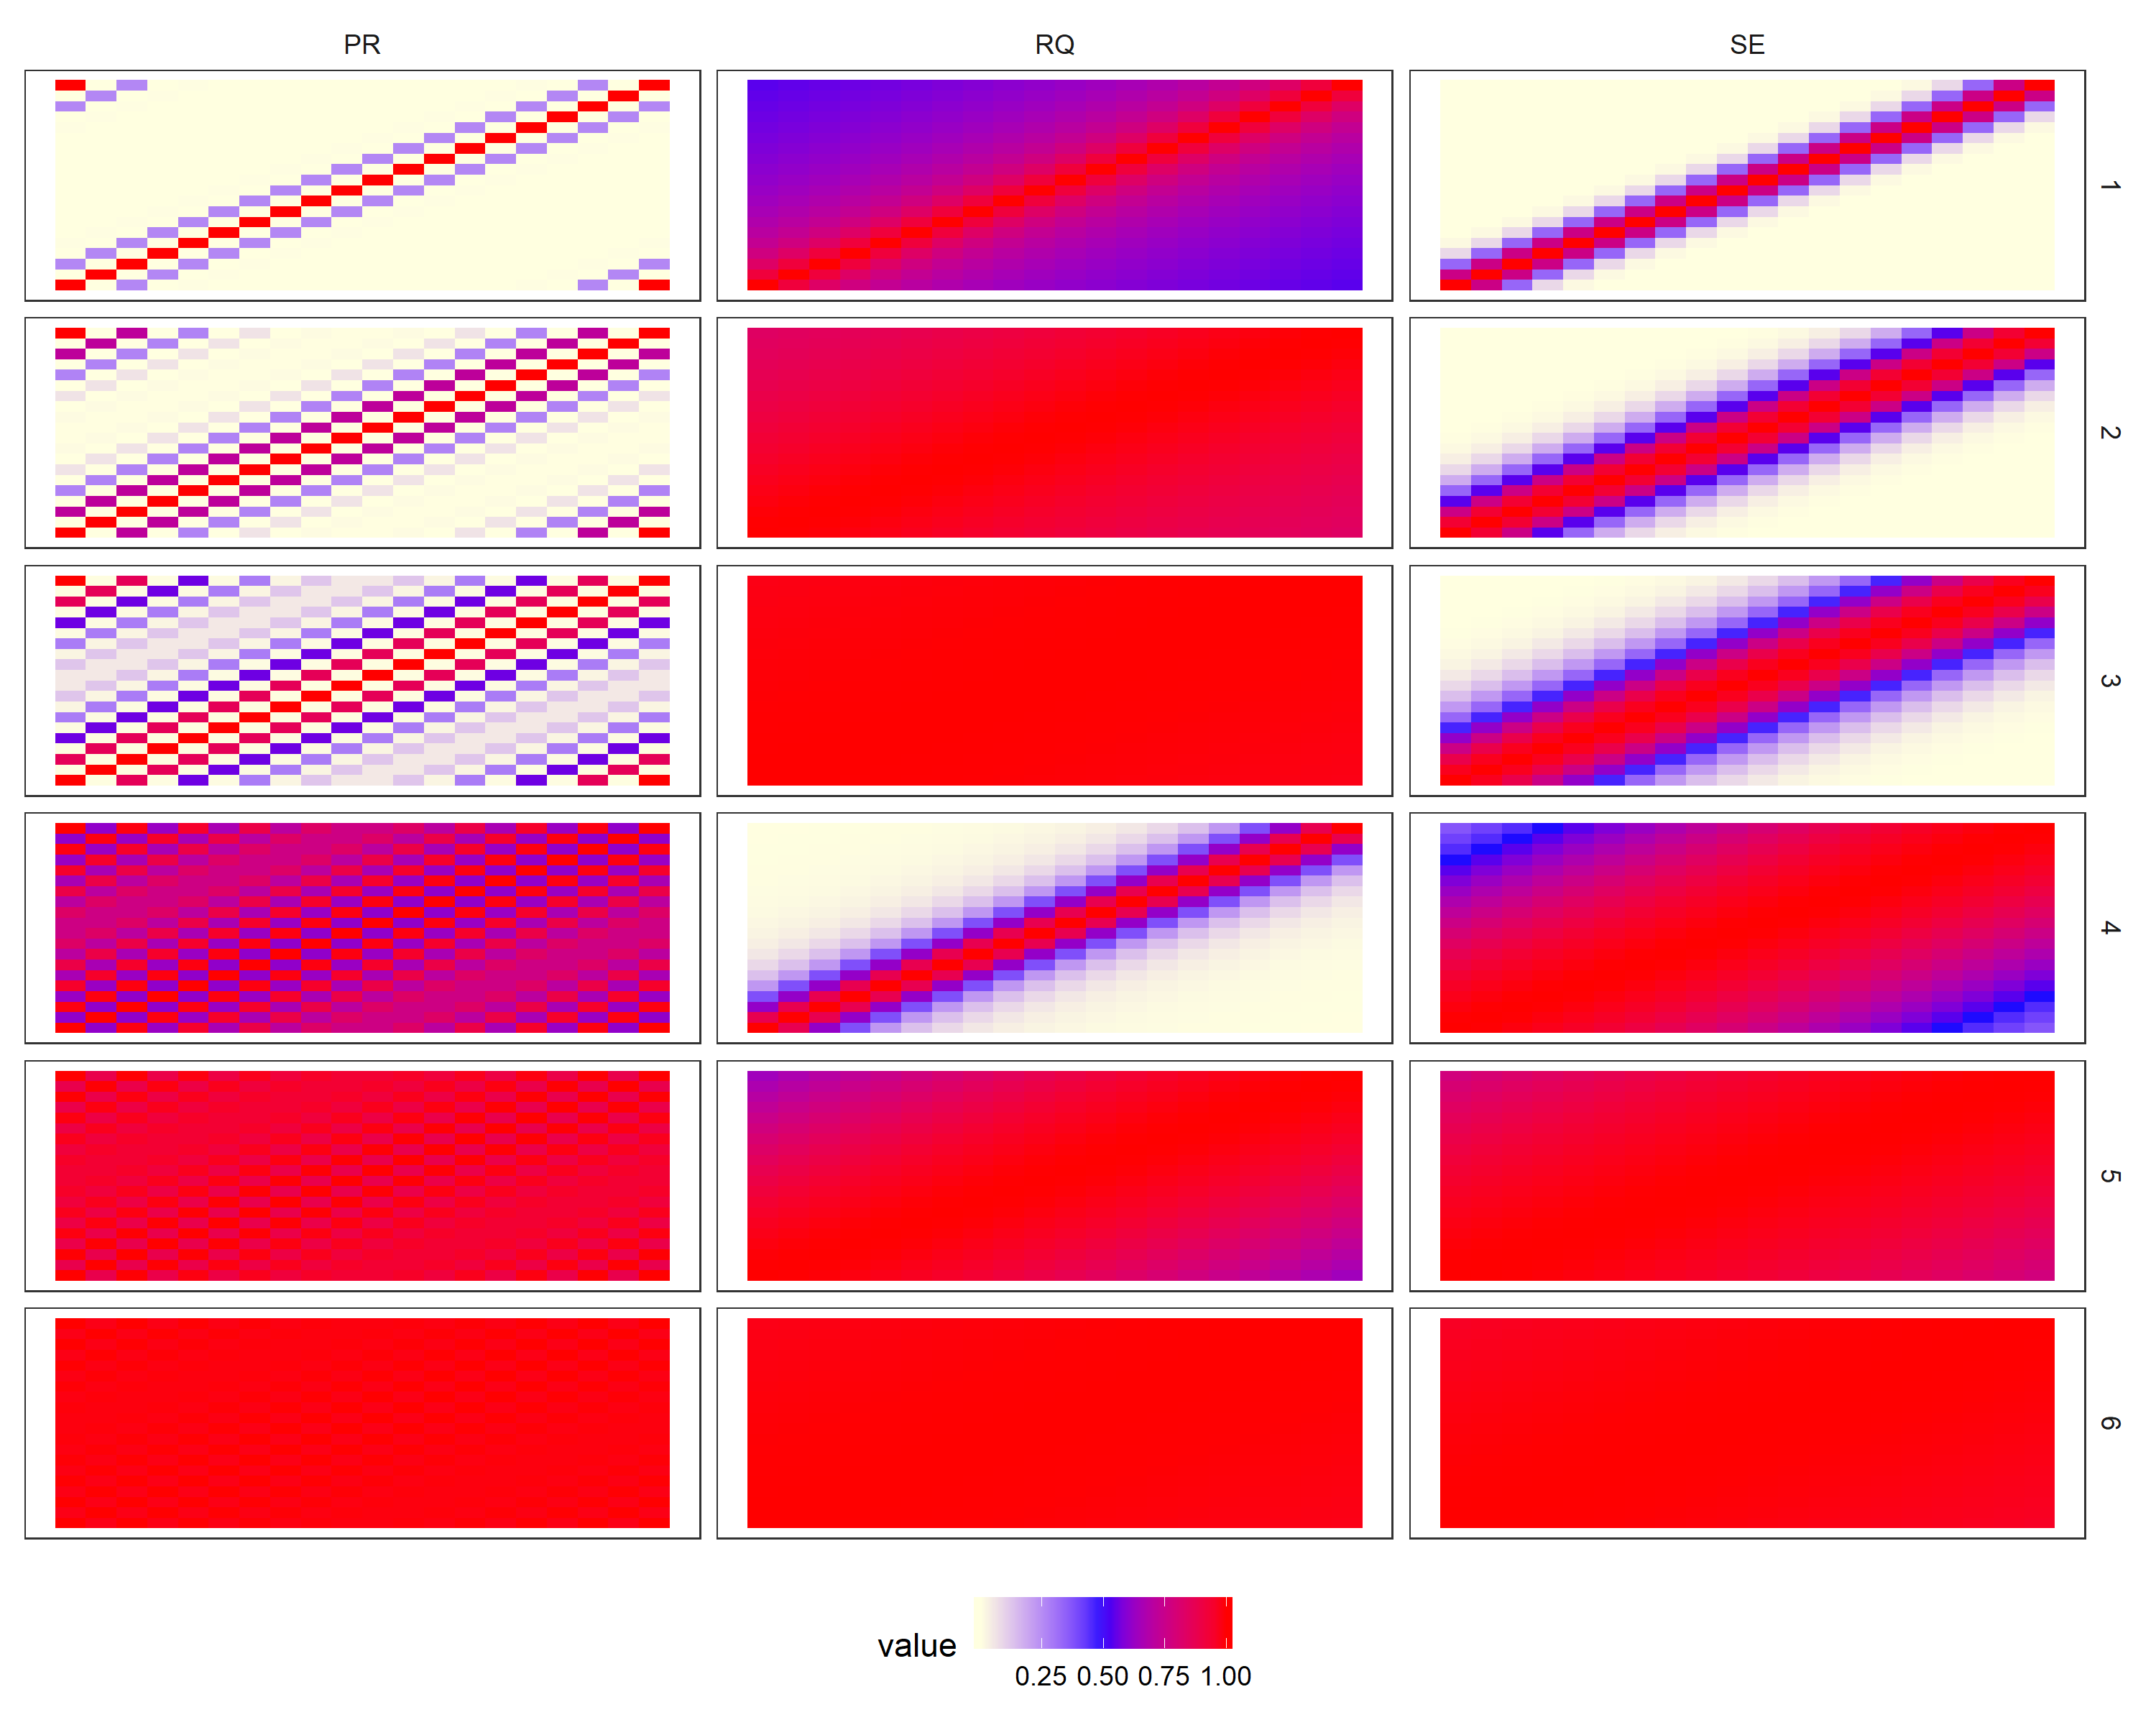
\includegraphics[scale = 0.15]{GP_illustrations/kernel_stationary.png}
\caption{Stationary kernels under 6 different sets of hyper-parameters.}\label{fig:}
\end{figure}

\begin{figure}[H]
\centering
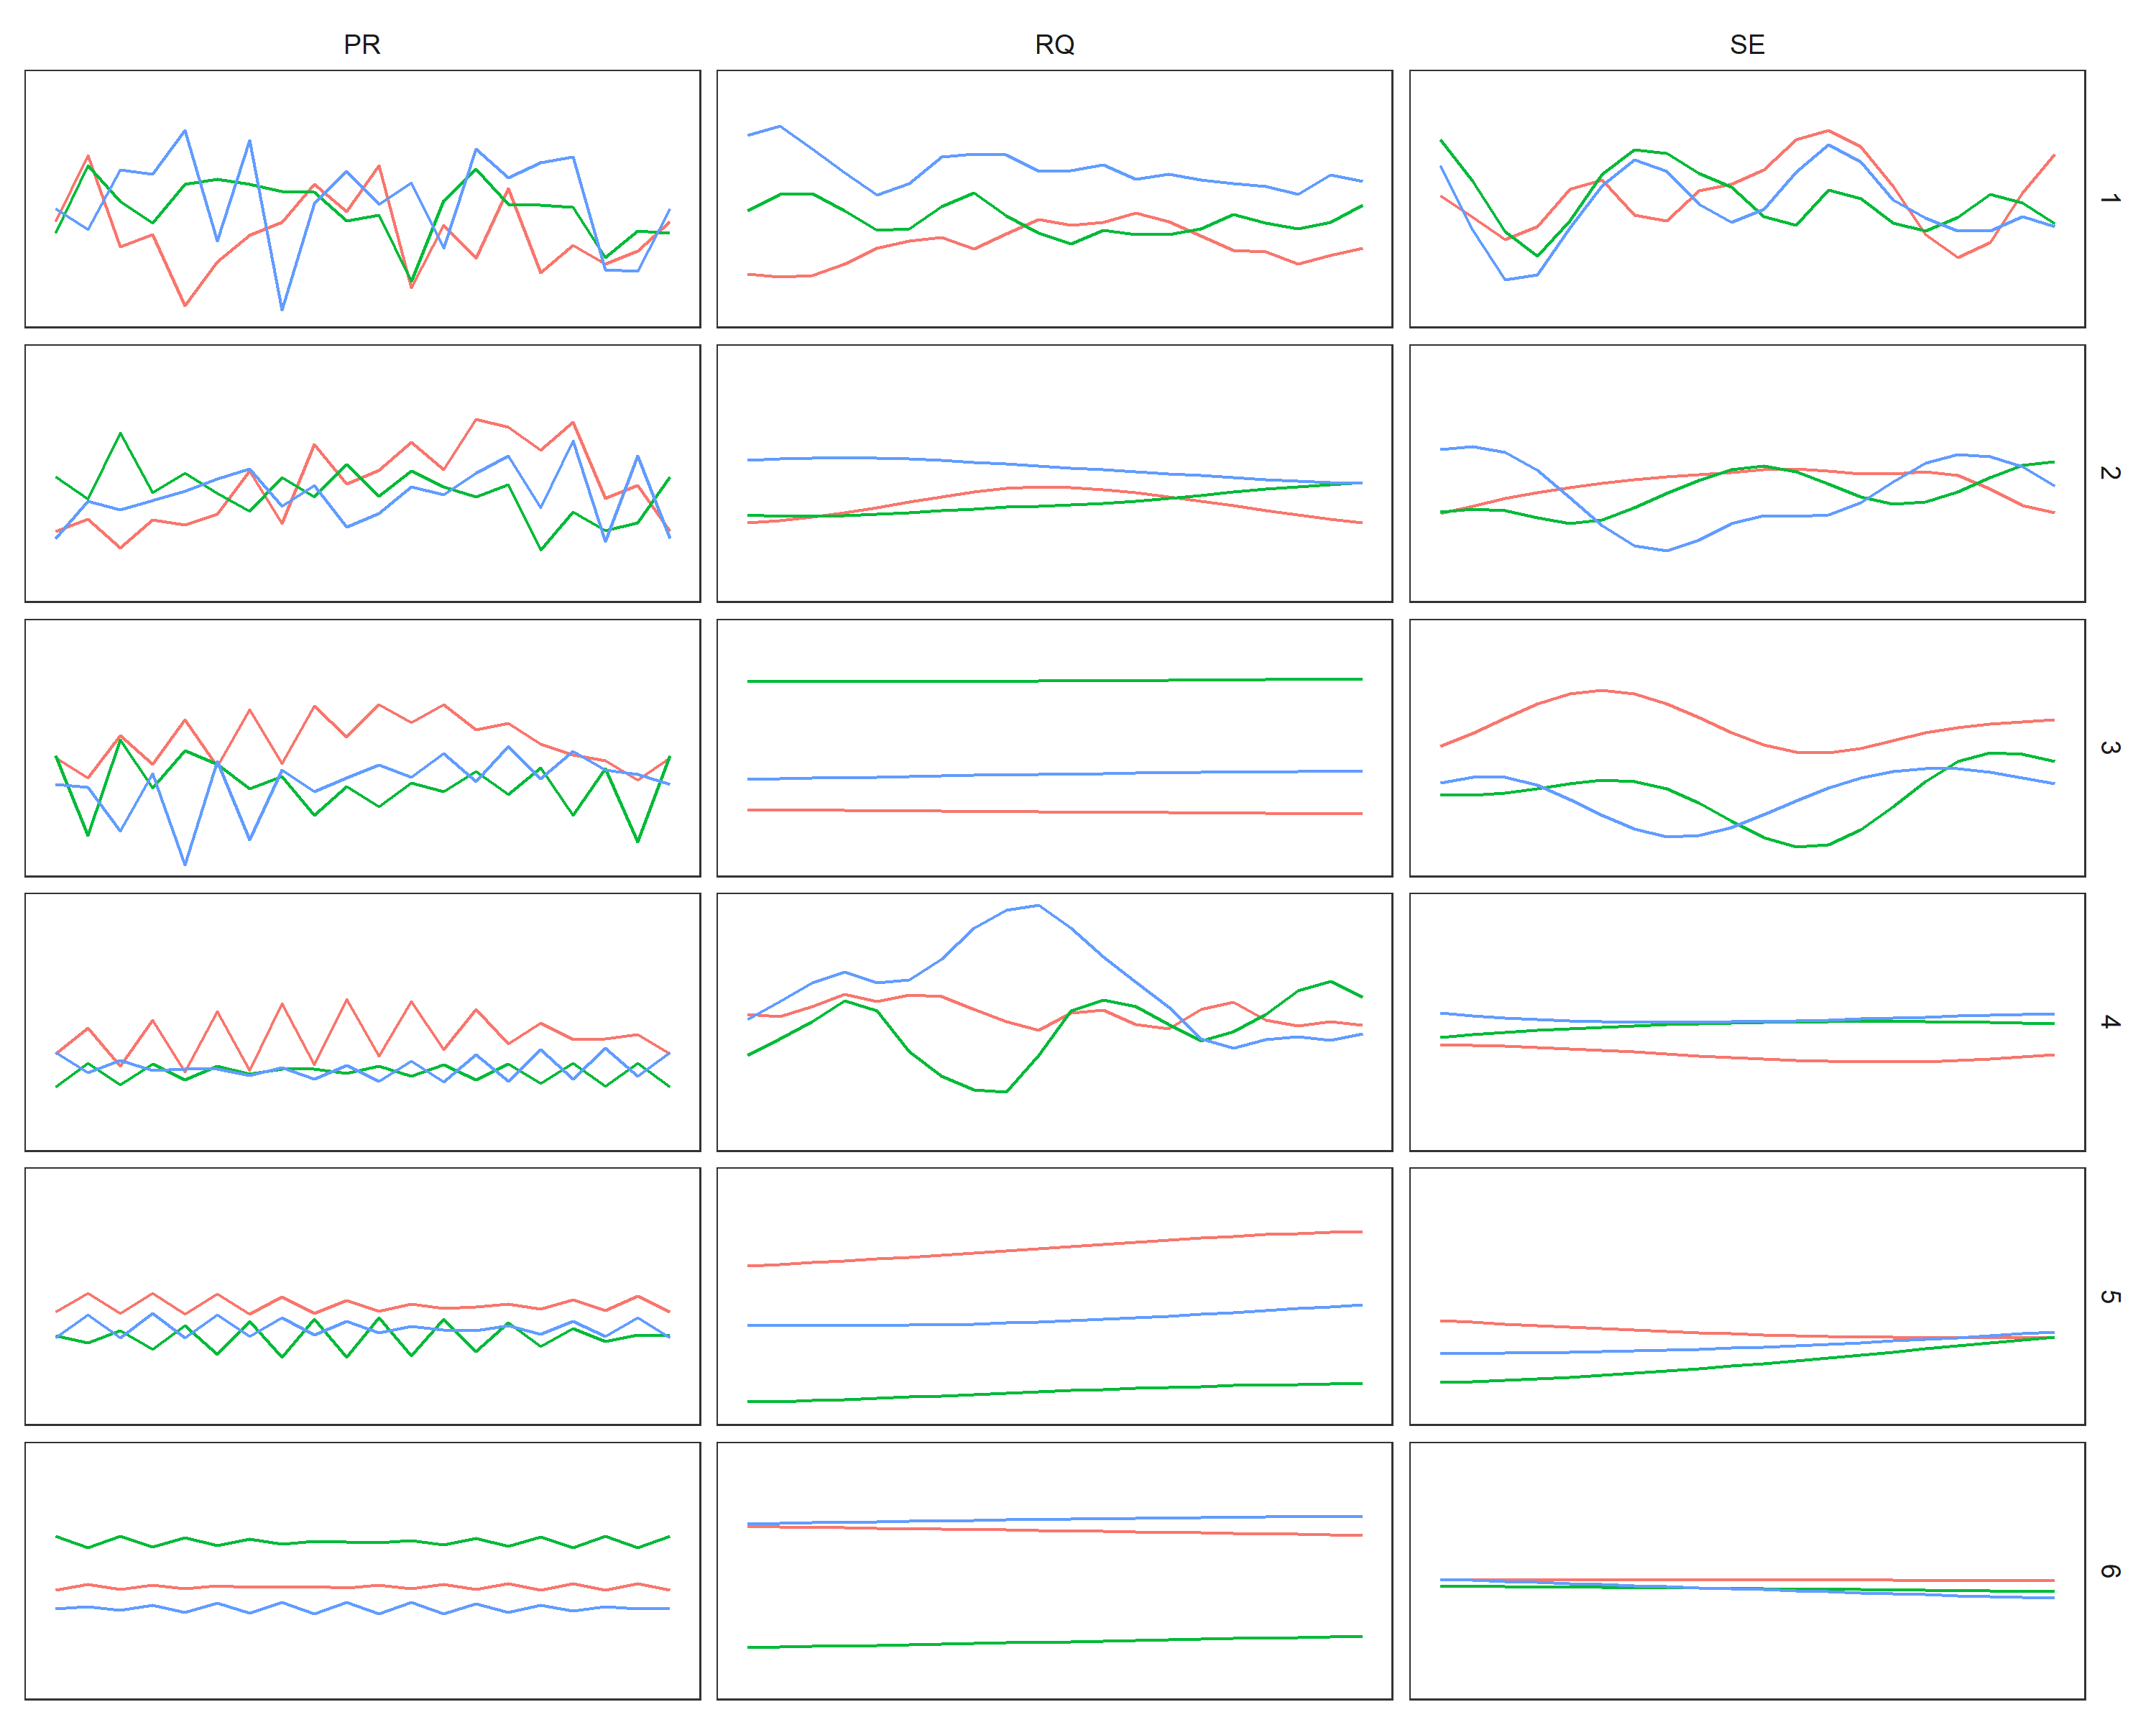
\includegraphics[scale = 0.15]{GP_illustrations/y_sim_stationary.png}
\caption{The 3 path of the signal $c_k$ simulated from the a priori distribution in Equation \eqref{eq:model_IMF_GP_k} under different stationary kernel assumptions (columns wise) and for 6 different sets of hyper-parameters.}\label{fig:}
\end{figure}

\begin{figure}[H]
\centering
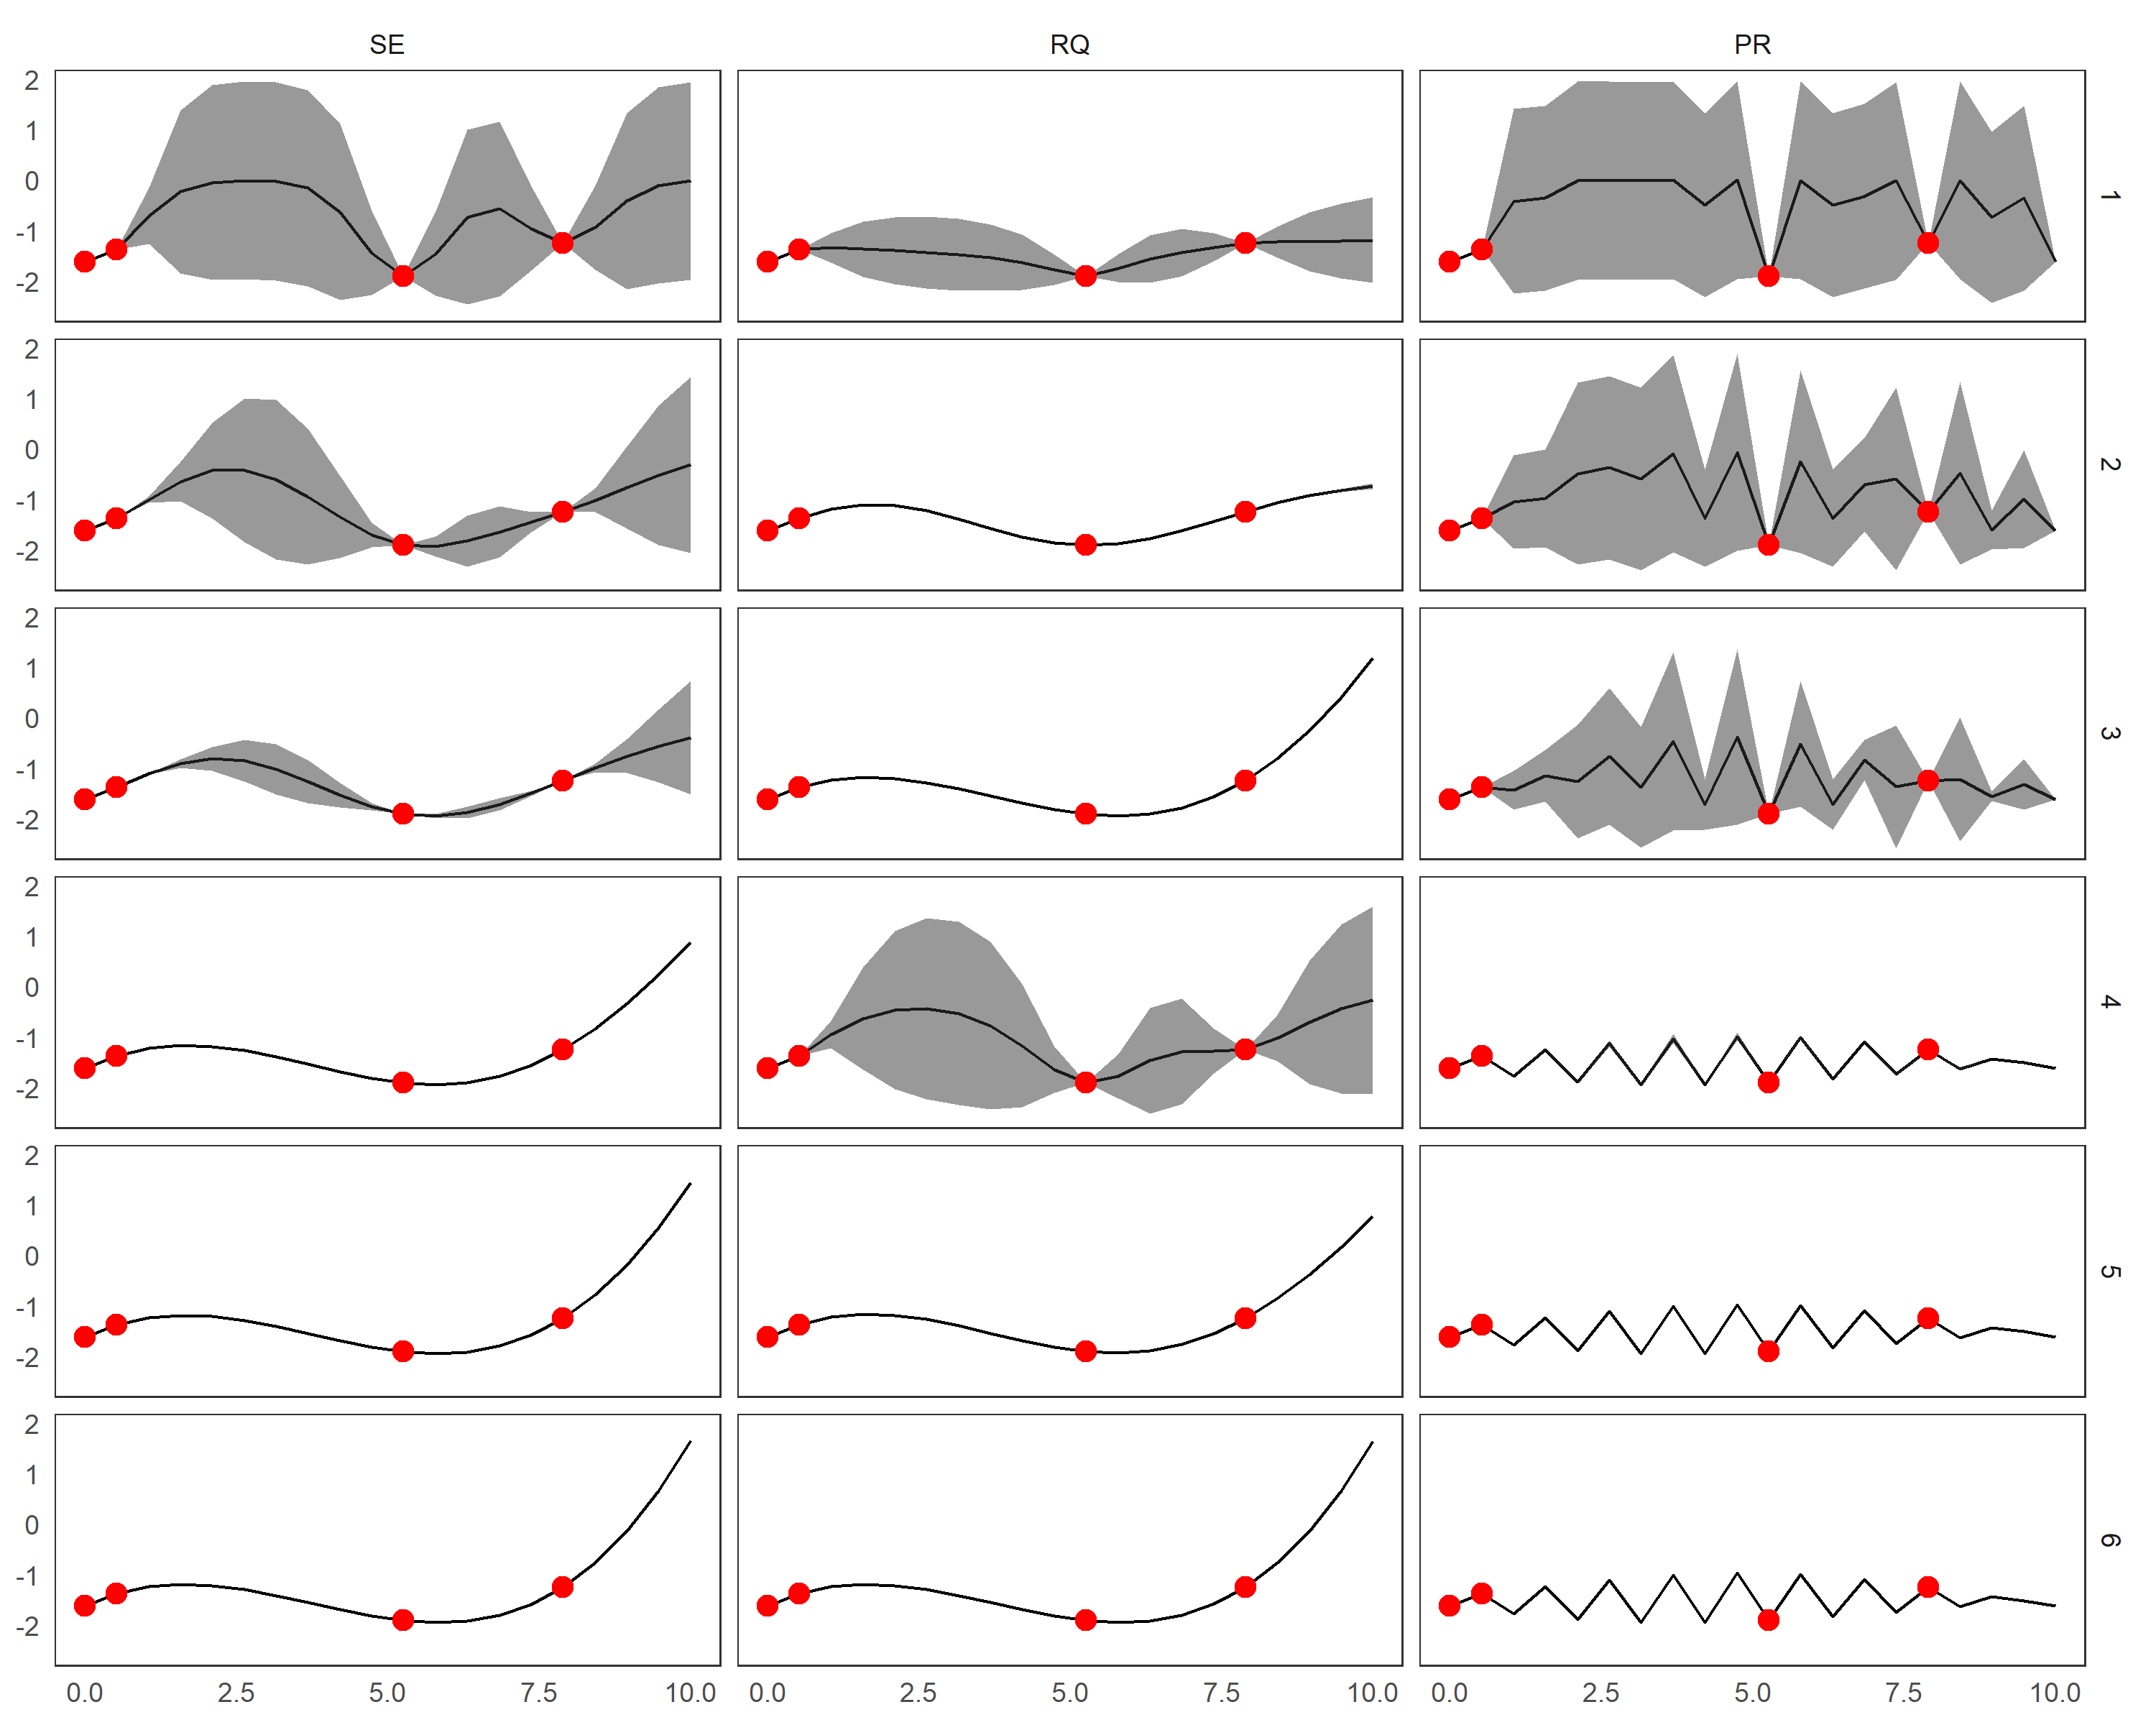
\includegraphics[scale = 0.15]{GP_illustrations/y_pred_stationary.png}
\caption{The predictive conditional mean of the IMF with the confidence intervals  under  noise-free assumption for different stationary kernel assumptions (columns wise) given 6 different sets of hyper-parameters. The red dots correspond to the observed values of the signal}\label{fig:}
\end{figure}